\chapter*{Introduction and Motivation}
\addcontentsline{toc}{chapter}{Introduction and Motivation}
\markboth{Introduction and Motivation}{Introduction and Motivation}
Inventory-aware market making balances execution revenue against the risk of holding a position. The classical Avellaneda--Stoikov formulation provides a useful benchmark for this trade-off under a stylized arrival model and exponential utility~\cite{as}. The first article in this series develops the classical comparison; the second introduces a finite-dimensional volatility lift and an inventory-control calculation on a scalar surrogate state~\cite{hft1,hft2}.

The present project asks a narrower question than whether a richer model produces better trading results: how much of the control equation is lost when the lifted state is compressed, and can this defect be corrected without evaluating a high-dimensional control problem online? A correction is useful only if its numerical and economic effects justify its computational cost. Lower residual alone is not evidence of better quotes, greater utility, or practical deployability.

This working draft establishes an operator-level foundation and reports an initial diagnostic of the inherited baseline. It does not yet contain a fitted correction, a converged reference HJB or a latency frontier. The manuscript is organized around these distinctions so that subsequent experiments can add evidence without changing the meaning of the reported quantities.

\chapter{From HFT2 to the Reduced-HJB Residual Problem}
\miniabstract{The series motivates a scalar policy for a multi-factor environment. This chapter defines what is compressed and separates model error from numerical error before any correction is fitted.}

Let $Z\in\mathbb R^M$ be the lifted volatility state and $Y=w^\top Z$ its aggregate. After separating cash and price under the assumptions specified in Chapter 3, write the certainty-equivalent adjustment as $\theta(t,q,Z)$. The reduced calculation replaces this object by $\theta_0(t,q,Y)$. Its embedding into the full state is
\[
 \widetilde\theta_0(t,q,Z)=\theta_0(t,q,w^\top Z).
\]
This is a composition of functions, not a statement that $Y$ is Markovian. In particular, the aggregate drift generally depends on the entire factor vector. Two states with the same $Y$ may therefore have different continuation dynamics.

\section{Two residuals and their difference}
For a specified full operator $\mathcal H_F$ and reduced operator $\mathcal H_R$, define
\[
 R_F=\mathcal H_F[\widetilde\theta_0],\qquad
 R_R=\mathcal H_R[\theta_0],\qquad D=R_F-R_R.
\]
The first quantity tests the embedded baseline against the full model. The second tests it against the equation it was intended to solve. The difference isolates the operator discrepancy only when all remaining terms, conventions and evaluation points agree. A large $R_F$ cannot be attributed to state compression if $R_R$ is already large.

For smooth scalar functions, the chain rule gives
\[
 \partial_{z_i}\widetilde\theta_0=w_i\theta_{0,y},\qquad
 \partial_{z_i z_j}\widetilde\theta_0=w_iw_j\theta_{0,yy}.
\]
These identities avoid a high-dimensional finite-difference grid for the initial diagnostic. They do not eliminate the need to validate the scalar derivatives, boundary treatment and time discretization. The first implementation interpolates previously computed scalar derivatives; it does not claim they are derivatives of a globally smooth interpolant.

The next chapter records the proposed correction architecture. Its role is to organize a research method; the financial operator itself is derived independently in Chapter 3.

\chapter{The Navier--Stokes Correction Architecture}
\miniabstract{The integration brief proposes a structural analogy built around residuals, correction families and localization. The source-specific correspondence remains pending until the exact Navier--Stokes document is available.}

The operational design follows the sequence: choose a background approximation, evaluate its full defect, decompose that defect, construct admissible corrections, localize them and recompute the complete nonlinear residual. This sequence is adopted as an algorithmic proposal. It is not supported here by a transfer of a fluid-mechanics theorem to a financial control problem.

\begin{center}\small
\begin{tabularx}{\textwidth}{@{}p{0.37\textwidth}X@{}}
\toprule
Construction described in the brief & Proposed HFT3 object \\
\midrule
Background field & Embedded scalar baseline $\widetilde\theta_0$ \\
Momentum residual & Full certainty-equivalent HJB defect $R_F$ \\
Stress representation & Decomposition into unresolved state directions \\
Covariance/wave families & Dictionary $\Phi_k$ of offline corrections \\
Positive-cone representation & Coefficients subject to justified admissibility constraints \\
Moment-restoring perturbations & Explicit preservation diagnostics for selected quantities \\
Cutoffs and localized support & Smooth correction gate $\chi$ \\
New nonlinear errors & Full residual recomputation after each stage \\
Complete correction cycle & Measured acceptance, rejection and stopping rules \\
\bottomrule
\end{tabularx}\end{center}

The exact document named in the integration brief has not yet been identified in the available project sources. Consequently, this table describes the requested research mapping rather than a verified account of a particular proof. Source verification must attach a page or section to each claimed construction and explain why its financial counterpart is well defined. Incompressibility, stress-tensor physics, blow-up statements and quantitative Navier--Stokes estimates are not imported.

Even if the source establishes a residual-improvement theorem in its own setting, an HJB correction needs separate assumptions, estimates and numerical evidence. In this project, improvement is initially an empirical acceptance criterion. The next chapter specifies the financial equation to which that criterion will be applied.

\chapter{Full Lifted Rough-Volatility HJB}
\miniabstract{The residual requires an explicit model. This chapter fixes a finite OU benchmark consistent with the inspected HFT2 code, including common factor noise, independent price noise and terminal liquidation.}

\section{State dynamics and objective}
Take positive decay rates $\lambda_i$ and deterministic weights $w_i$. The inherited finite-factor benchmark is
\[
 dZ_t^{(i)}=-\lambda_i Z_t^{(i)}dt+dB_t,\qquad
 Y_t=\sum_{i=1}^M w_iZ_t^{(i)},\qquad
 dS_t=\sqrt{v(Y_t)}\,dW_t,
\]
where the same Brownian motion $B$ drives every factor and $W$ is independent of $B$. Thus the instantaneous factor covariance is $\mathbf1\mathbf1^\top$, not the identity. Under stationary initialization,
\[
 \Sigma_{ij}=\frac1{\lambda_i+\lambda_j},\quad
 s_Y^2=w^\top\Sigma w,\quad
 v(y)=\sigma_0^2\exp\!\left(\beta y-\tfrac12\beta^2s_Y^2\right).
\]
The exact one-step innovation covariance is
\[
 Q_{ij}(h)=\frac{1-\exp[-(\lambda_i+\lambda_j)h]}{\lambda_i+\lambda_j}.
\]
Independent factors would represent a different model. The finite exponential mixture is a benchmark approximation; this draft does not establish a calibrated power-law limit or a Hurst-parameter interpretation beyond the inherited weight rule.

Inventory $q\in\{-Q,\ldots,Q\}$ changes by one unit on a fill. Bid and ask offsets $\delta^b,\delta^a$ have arrival intensities $A e^{-k\delta}$. At the inventory limits, the side that would violate the constraint is disabled. The terminal cash-equivalent liquidation cost is
\[
 L(q,y)=(\ell_1+\ell_v\sqrt{v(y)})|q|+\ell_2q^2.
\]
The objective is exponential utility of terminal marked-to-market wealth less $L$, with risk aversion $\gamma>0$. Under price translation invariance and independent price/factor noise, use
\[
 U(t,x,s,q,z)=-\exp\{-\gamma[x+qs+\theta(t,q,z)]\},
 \qquad \theta(T,q,z)=-L(q,w^\top z).
\]
Here $U$ is utility and $\theta$ is a certainty-equivalent adjustment. Applying the nonlinear operator to one while interpreting it as the other would change the residual.

\section{The operator and bounded controls}
Set $b_i(z)=-\lambda_i z_i$, $a=\mathbf1\mathbf1^\top$, and
\[
 h(d)=\max_{\delta\in[\delta_{\min},\delta_{\max}]}
 \frac{A e^{-k\delta}}\gamma\left[1-e^{-\gamma(\delta+d)}\right].
\]
The maximizing quote, for this declared admissible interval, is
\[
 \delta^*(d)=\operatorname{clip}\!\left(
 \frac{\log(1+\gamma/k)}\gamma-d,
 \delta_{\min},\delta_{\max}\right).
\]
Substitution of the utility ansatz into the diffusion and jump generator yields
\begin{align*}
 \mathcal H_F[\theta]={}&\theta_t+b^\top\nabla\theta
 +\tfrac12\operatorname{tr}(a\nabla^2\theta)
 -\tfrac\gamma2\nabla\theta^\top a\nabla\theta
 -\tfrac\gamma2q^2v(w^\top z)\\
 &+\mathbf1_{q<Q}h(\theta(t,q+1,z)-\theta(t,q,z))\\
 &+\mathbf1_{q>-Q}h(\theta(t,q-1,z)-\theta(t,q,z)).
\end{align*}
The equation is $\mathcal H_F[\theta]=0$. The negative gradient-square term comes from differentiating the exponential utility ansatz. The common factor driver requires all mixed Hessian entries. If price/factor correlation is introduced later, additional cross terms must be derived before reusing this operator.

The inherited HFT2 solver uses an unconstrained arrival Hamiltonian and clips evaluated quotes afterwards. The present diagnostic uses the bounded Hamiltonian on both sides of the residual comparison, with interval $[0.02,4]$. It therefore evaluates a declared admissible-control problem rather than silently identifying the two implementations. This difference must be resolved in the next baseline solver.

\chapter{Residual Decomposition of State Compression}
\miniabstract{With identical volatility and arrival terms, the difference between full and scalar operators has an explicit drift and diffusion decomposition. This gives a testable starting point for selecting correction directions.}

The scalar surrogate uses drift $-\kappa y$ and diffusion variance $\eta^2$. Applying the chain rule from Chapter 1 gives
\begin{align*}
 D(t,q,z)={}&\left[\kappa y-\sum_iw_i\lambda_i z_i\right]\theta_{0,y}\\
 &+\frac12\left[\left(\sum_iw_i\right)^2-\eta^2\right]
 \left(\theta_{0,yy}-\gamma\theta_{0,y}^2\right).
\end{align*}
This identity assumes the same time derivative, variance map, inventory boundaries and Hamiltonian on both sides. It is an operator identity for a sufficiently smooth baseline, not an error estimate for a numerical solution.

In the inspected HFT2 defaults, $M=6$, rates span $3$ to $180$, weights sum to one, and $\kappa=1.35$. The scalar diffusion is chosen to match stationary variance: $\eta^2=2\kappa s_Y^2$. This does not also match the full aggregate's instantaneous variance, which is $(\sum_iw_i)^2=1$. Matching a stationary moment is therefore insufficient to identify a local generator.

The drift mismatch suggests directions orthogonal to the scalar aggregate, while the diffusion mismatch already acts on scalar derivatives. A low-rank dictionary should be selected from evaluated defects, not only from the decay-rate ordering. A fast/slow parameter such as $\varepsilon=\lambda_{\rm slow}/\lambda_{\rm fast}$ is meaningful only after groups and an approximation regime have been specified. No asymptotic limit is established here.

The next two chapters describe how these directions can enter a correction while preserving the terminal condition and maintaining control over the full residual.

\chapter{Correction Families and Preservation Constraints}
\miniabstract{Correction functions are represented independently of the operator. This makes it possible to test their derivatives and boundary behavior before fitting coefficients to a residual.}

Consider a finite family $\Phi_1,\ldots,\Phi_K$ and $C=\sum_k c_k\Phi_k$. A candidate offline fit minimizes a weighted residual objective on training points, subject to declared admissibility constraints. A separate evaluation set is required: reducing the fitted residual on the same points used to choose the coefficients would provide weak evidence of approximation quality.

One useful structural condition is $\Phi_k(T,q,z)=0$, which preserves the prescribed terminal value exactly. This is distinct from preserving a statistical moment. Inventory monotonicity, signs of quote offsets and coefficient positivity are possible constraints, but they must follow the chosen control problem rather than a formal analogy with a cone in another domain.

Moment preservation also requires a precise object. Correcting a value function without changing the exogenous factor dynamics leaves the factor covariance unchanged automatically. Such a check is necessary for implementation integrity but is not evidence that the policy preserves liquidation risk. A nontrivial economic constraint would concern quantities affected by the policy, such as a selected terminal inventory statistic, evaluated under a common simulation design.

The implemented interface represents a value and its time, gradient, Hessian and neighboring-inventory values. It supports composition and addition of corrections. The coefficient optimizer and the data-driven dictionary remain research tasks. Before optimizing them, localization must be included in the derivative calculation.

\chapter{Localized Iterative HJB Correction}
\miniabstract{A local correction changes both the approximation and its derivatives. The implementation therefore carries complete product derivatives and reevaluates the nonlinear operator after every proposed update.}

Let a gate $\chi\in[0,1]$ activate a correction in selected regions. Define
\[
 \theta_{j+1}=\theta_j+\chi_j C_{j+1},\qquad
 R_{j+1}=\mathcal H_F[\theta_{j+1}].
\]
For the product $F=\chi C$, spatial derivatives satisfy
\[
 \nabla F=C\nabla\chi+\chi\nabla C,
\]
\[
 \nabla^2F=C\nabla^2\chi+\chi\nabla^2C
 +\nabla\chi\nabla C^\top+\nabla C\nabla\chi^\top.
\]
Dropping the last two terms would change the full residual exactly where the gate transitions. The same product rule applies to time derivatives, and the gate must be evaluated at neighboring inventories for the arrival terms.

The first gate implementation uses the quintic transition
\[
 s(x)=10x^3-15x^4+6x^5,\qquad 0<x<1,
\]
extended by zero and one outside this interval. Its first two derivatives vanish at the endpoints, so the extended gate is $C^2$. A state-coordinate transformation used as its argument must itself supply the necessary derivatives.

A step may be accepted when the evaluated residual norm decreases by a prescribed factor and all constraints remain satisfied. Successful acceptance is not the same as stopping. Termination needs an absolute tolerance, a maximum cycle count, stagnation detection or an explicit cost budget. Zero initial residual and zero cost increment require separate handling. No contraction theorem or fitted iterative cycle is claimed by the current implementation.

\chapter{Low-Latency C++ Realization}
\miniabstract{The first code increment establishes the offline residual evaluator and derivative-aware correction interfaces. It does not yet replace the starter's artificial quote surfaces with a solved policy.}

The offline path evaluates the full operator, fits corrections and exports policy surfaces. The online target is a fixed-size factor update, aggregation, baseline lookup, gate evaluation and a small bounded number of correction lookups. The state recurrence alone costs $O(M)$. Exact correlated OU innovation generation with a dense precomputed factor costs $O(M^2)$ per simulation step; its factorization costs $O(M^3)$ offline. Correction cost also includes feature construction and support selection. These components must be timed separately before assigning a complexity or latency to the complete decision. The offline Hessian contraction currently costs $O(M^2)$; it is not part of the online latency claim.

The first implementation provides a bounded arrival Hamiltonian, a common-noise full residual evaluator, scalar-to-vector derivative embedding, a smooth gate and exact correction-product derivatives. Parameters and diagnostic inputs are validated. Arithmetic overflow in the residual is reported instead of silently clipping it. Tests cover inventory limits, quote optimization against a grid search, mixed Hessian terms, scalar embedding, gate derivatives and nonlinear recomputation.

The original demonstration still uses synthetic surfaces without a time coordinate. A finite-horizon solved policy must represent the remaining time explicitly or use an equivalent validated selection of time slices. It would be misleading to report the starter's lookup as the performance of the future corrected HJB policy.

Software timing will be measured separately for factor updates, baseline lookups, corrections and the complete decision. Warm-up, timer overhead, repeated trials, compiler flags and hardware disclosure are prerequisites. No exchange round-trip claim follows from a local microbenchmark. The next chapter reports only the checks actually completed in this increment.

\chapter{Initial Numerical Audit}
\miniabstract{The initial experiment is a baseline diagnostic and a cross-language check. It is not a corrected-policy comparison and does not establish convergence of the inherited solver.}

The audit imports the inspected HFT2 source without modifying it and runs its default scalar solver for $H=0.2$. Synthetic stationary lifted states are sampled with seed 42. Evaluation uses time indices $0$, $195$ and $388$, five inventory levels and twelve states per combination, producing 180 interior samples. Time differentiation is forward, spatial differences follow the inherited solver and derivative values are linearly interpolated.

\begin{center}
\begin{tabular}{@{}lr@{}}
\toprule
Diagnostic & Value \\
\midrule
Full aggregate instantaneous variance & $1.000000$ \\
Reduced diffusion variance & $0.209552$ \\
Full residual RMS & $138562.58$ \\
Reduced residual RMS & $113726.58$ \\
Operator-difference RMS & $38015.32$ \\
Pre-terminal entries at lower clip $-60$ & $6514$ \\
Pre-terminal entries at upper clip $15$ & $159144$ \\
\bottomrule
\end{tabular}
\end{center}

These unnormalized values are diagnostics under the declared discretization and bounded Hamiltonian. The inherited solver clips its value array and uses a different, unconstrained arrival term. Both choices matter when interpreting the residual. Entries at clipping bounds do not by themselves identify the cause of the numerical behavior, but the combination of extensive saturation and a large reduced residual rules out treating this run as a validated converged baseline.

An independent C++ evaluation agrees with the exported Python residuals on all 180 samples within the prescribed relative tolerance $10^{-9}(1+|R|)$. The deterministic test executable passes 528 checks. These results verify implemented arithmetic and selected interfaces; they do not validate an optimal policy or justify a correction fit on the saturated baseline.

\section{A positive transformed baseline}
To address this issue, the next implementation uses $u=\exp(-\gamma\theta)>0$. On the scalar state grid its equation is
\begin{align*}
0={}&u_t+\mathcal L_Ru+\tfrac12\gamma^2q^2v(y)u\\
 &+\sum_{\pm}\min_{\delta\in[0.02,4]}
 Ae^{-k\delta}\bigl(e^{-\gamma\delta}u_{q\pm1}-u_q\bigr),
\end{align*}
where forbidden inventory transitions are omitted. The terminal condition is $u(T,q,y)=\exp(\gamma L(q,y))$. The transformation removes the spatial gradient-square term; it does not remove the coupled control optimization over neighboring inventories.

For spacing $h$, use nonnegative state-transition rates
\[
 a_-={\eta^2\over2h^2}+{\max(-b,0)\over h},\qquad
 a_+={\eta^2\over2h^2}+{\max(b,0)\over h},\qquad b=-\kappa y.
\]
Outward state transitions are suppressed at the two truncated boundaries. Each backward explicit step uses the minimizing quotes computed from the current positive array. The condition
\[
 \Delta t\left(a_-+a_++2Ae^{-k\delta_{\min}}\right)<1
\]
is sufficient for nonnegative coefficients in each controlled step; the inventory-risk term adds a nonnegative diagonal contribution. This gives an algebraic positivity property of the scheme. It is not a proof of convergence to the unbounded-domain HJB. Domain truncation, consistency, time error and policy error still require study.

The implementation chooses substeps from a conservative global bound with safety factor $0.8$. It reports a failure if a transformed value becomes nonpositive or nonfinite; no clipping of $\theta$ is used. Deterministic tests pass for a constant solution, an analytic no-arrival constant-volatility limit, inventory symmetry, positivity and invalid grids.

\begin{center}
\begin{tabular}{@{}rrrr@{}}
\toprule
State points & Time steps & $\theta(0,0,0)$ & $\theta(0,2,0)$\\
\midrule
61 & 2340 & 6.701053 & 6.367267\\
61 & 4680 & 6.699587 & 6.365723\\
121 & 2340 & 6.701135 & 6.367370\\
121 & 4680 & 6.699669 & 6.365826\\
241 & 2340 & 6.701176 & 6.367421\\
241 & 4680 & 6.699709 & 6.365878\\
\bottomrule
\end{tabular}
\end{center}
All six runs keep $u$ positive. With 4680 time steps, the change in $\theta(0,0,0)$ from 121 to 241 points is approximately $4.08\times10^{-5}$; halving the time step at 241 points changes it by approximately $1.47\times10^{-3}$. These are selected-point refinement diagnostics, not global error bounds. These initial runs exported only time-zero values. The following experiment extends the export to physical-time slices and examines joint domain/grid sensitivity; independent residual validation remains open.

\section{Time-dependent policies and domain sensitivity}
The next increment retains 41 physical-time slices, including both endpoints, from each backward solve. Nine configurations combine 81, 161 and 241 state nodes with symmetric domains of four, five and six stationary standard deviations. All use 9360 actual time steps. These are discretizations of the same scalar model, not nine market models or simulated trading sessions. The CSV export contains 772317 state-time-inventory records. An unavailable quoting side at an inventory limit is stored as missing, not as a zero offset.

Figure~\ref{fig:temporal-policy} shows the solved baseline at three times. The rows expose the approach to the liquidation condition; the columns distinguish the certainty equivalent from executable offsets. Inventory is discrete, so horizontal bands are expected. White boundary rows mark forbidden trades. The color scales are local to each panel. Near the terminal time, aggressive offsets can reach the declared lower bound; this is a control constraint, not clipping of the value function.

\begin{figure}[p]
\centering
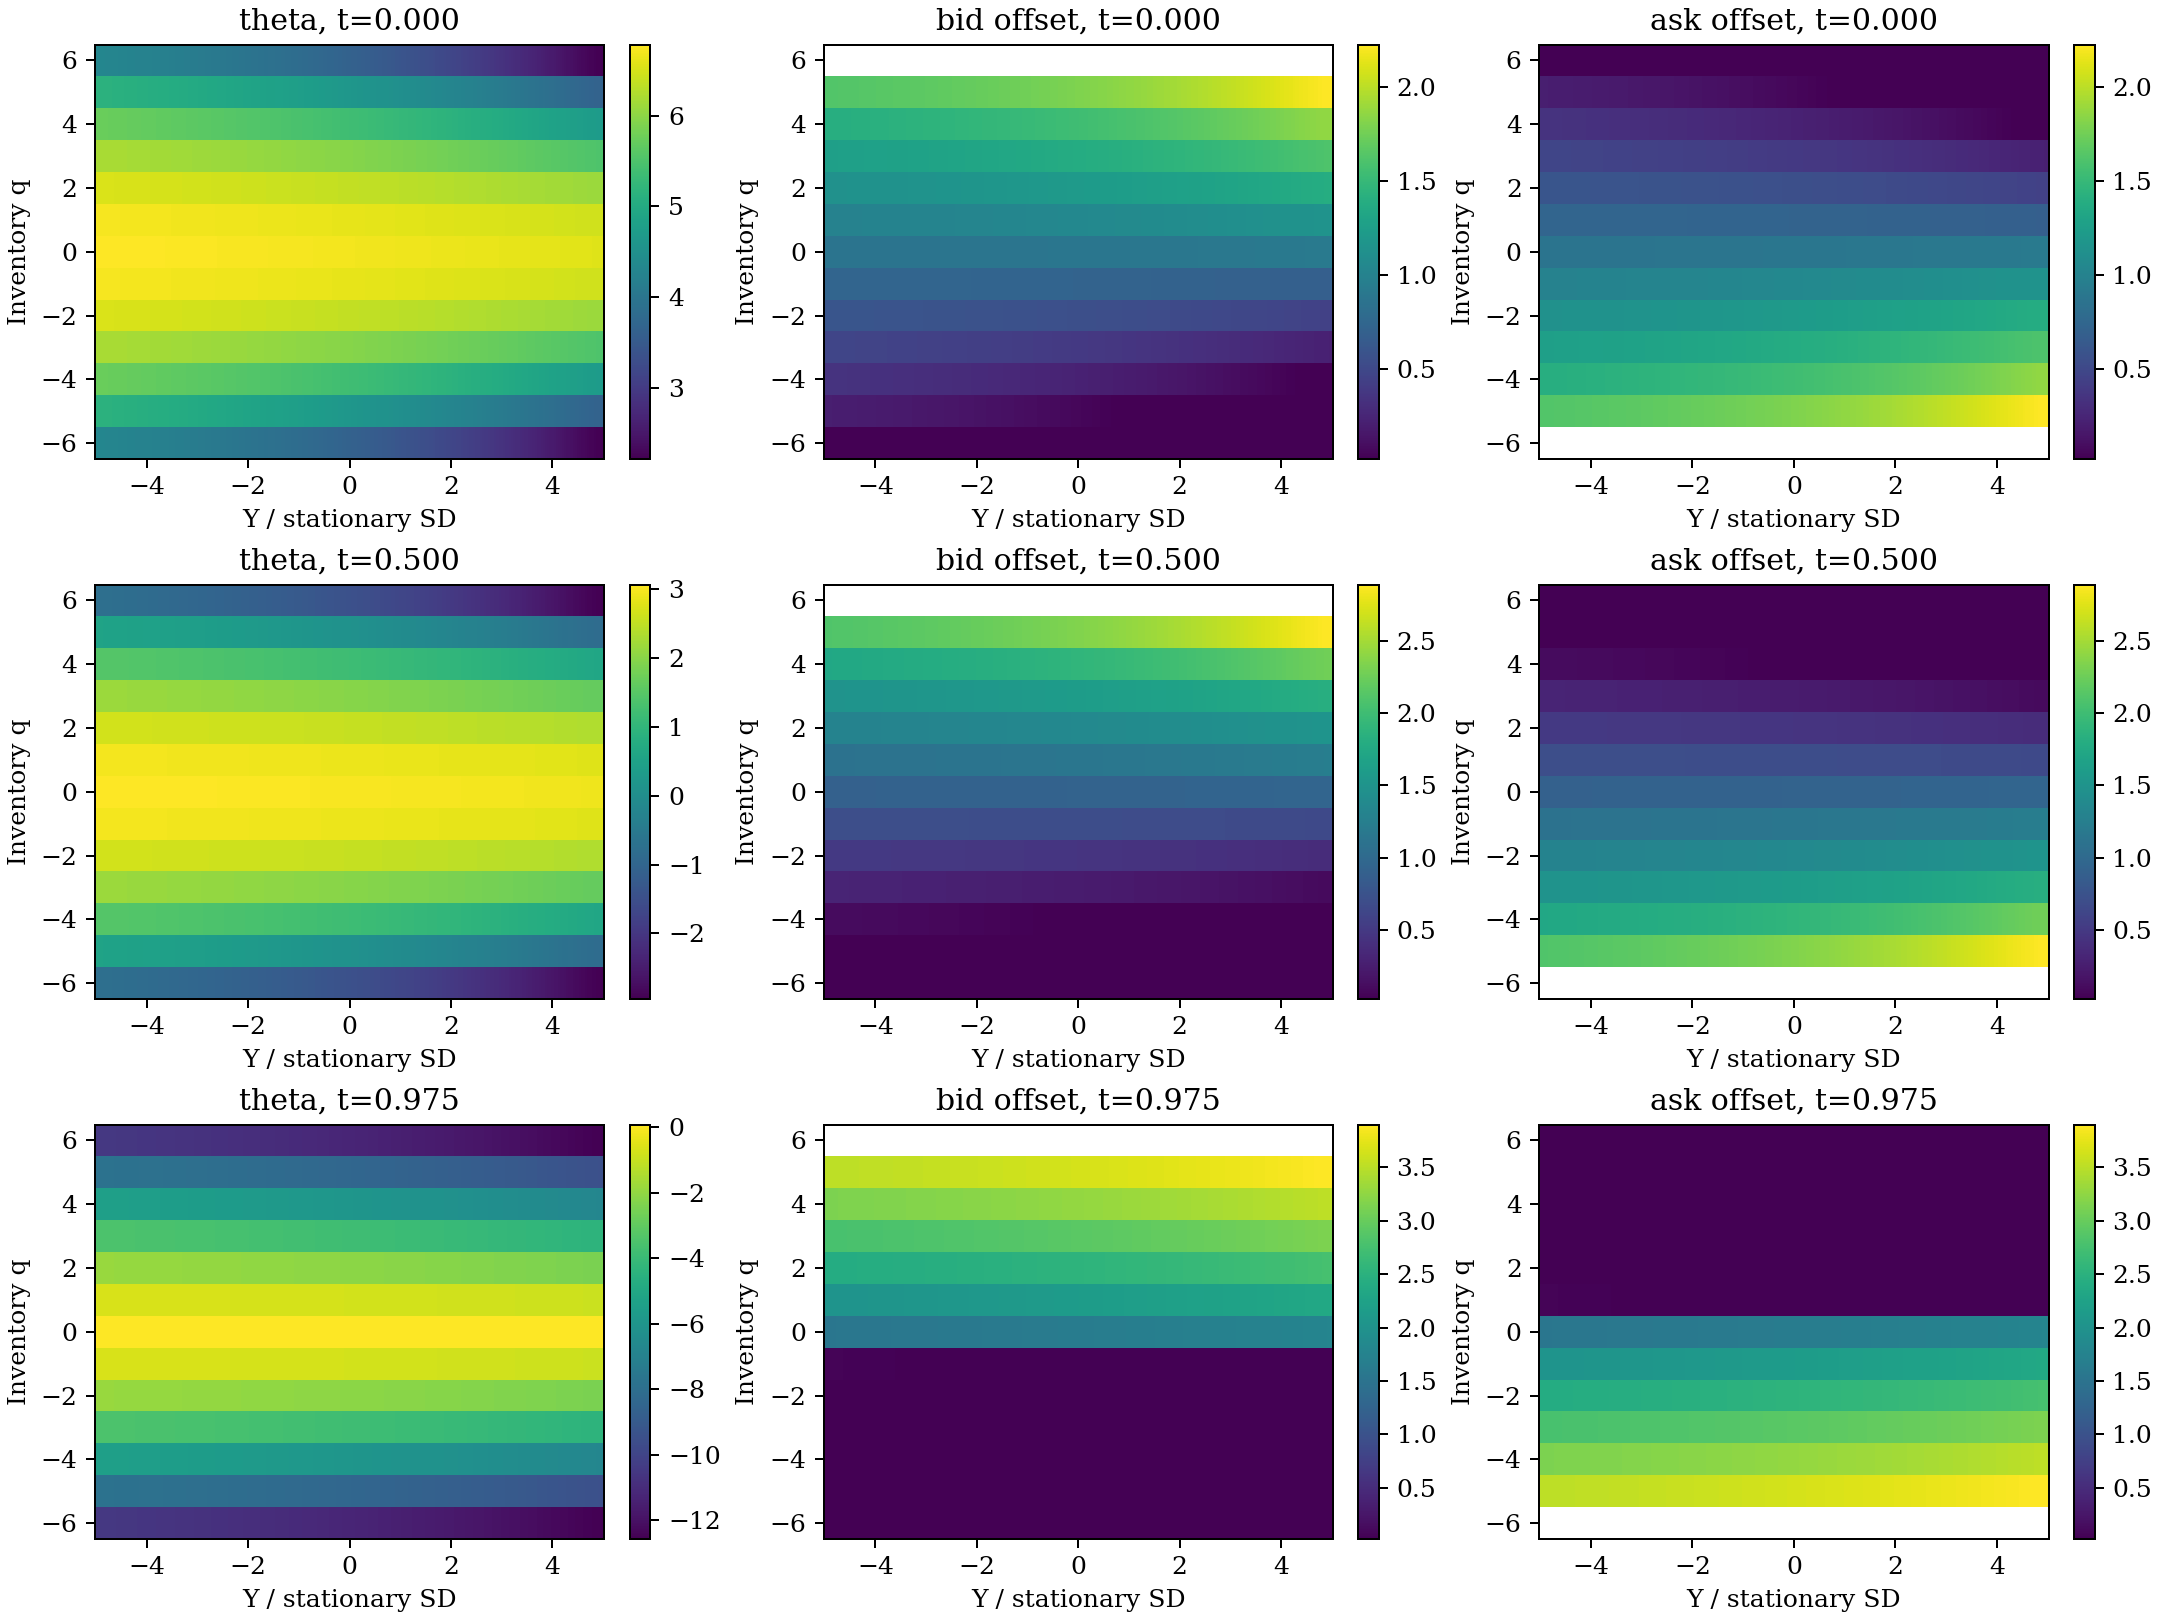
\includegraphics[width=\textwidth]{img/temporal_policy.png}
\caption{Solved scalar baseline: certainty equivalent and bid/ask offsets at $t=0$, $0.5$ and $0.975$, with $T=1$. Domain $\pm5$ stationary standard deviations, 241 state nodes, 9360 steps. Values and offsets use the model's monetary/price units; time is normalized. Blank cells denote disabled sides at inventory limits. Deterministic HJB computation, not Monte Carlo.}
\label{fig:temporal-policy}
\end{figure}

The export checks recover the terminal condition with maximum absolute error $5.33\times10^{-15}$, and all available offsets remain in $[0.02,4]$. Additional C++ tests verify temporal ordering, endpoint inclusion, the analytic no-arrival risk limit at every saved time, and exact agreement between the final snapshot and the existing time-zero API. Exporting the history does not change the numerical evolution.

Figure~\ref{fig:policy-sensitivity} compares all saved times, inventory levels and admissible sides on 101 common points in $|Y|\leq2\sqrt{\operatorname{Var}(Y)}$. Linear interpolation maps each grid to these points. The six-standard-deviation, 241-node run is a comparison surface, not an exact solution. Across the configurations, maximum differences are approximately $1.62\times10^{-3}$ for the value and $1.15\times10^{-3}$ for offsets. The zero at the reference configuration is an identity, not evidence of zero numerical error.

\begin{figure}[htbp]
\centering
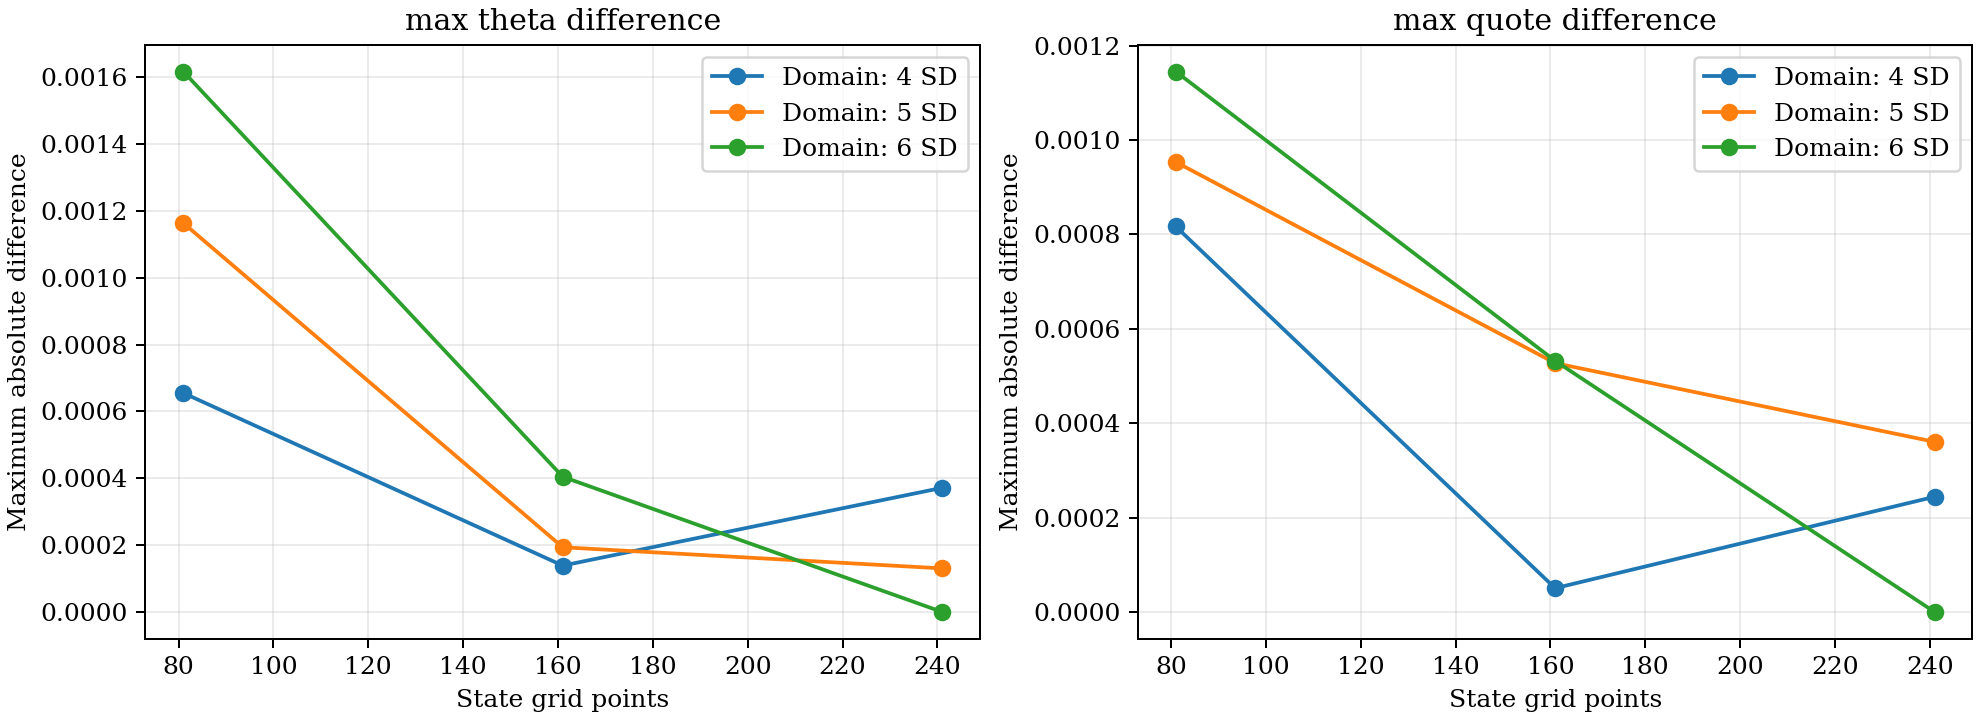
\includegraphics[width=\textwidth]{img/policy_sensitivity.png}
\caption{Joint grid/domain sensitivity relative to the six-standard-deviation, 241-node run, at a common 9360 time steps. Maxima cover all 41 saved times and the central two-standard-deviation interval. Changing the domain at fixed node count also changes spacing; the nonmonotone four-standard-deviation curve cannot be interpreted as an isolated boundary error.}
\label{fig:policy-sensitivity}
\end{figure}

The computational purpose of precomputation is to move HJB evolution outside the decision loop. Saving selected slices costs memory proportional to the number of stored times, inventory levels and state nodes, rather than requiring every solver step to be retained. This increment supplies offline CSV data; a validated online interpolator and a measured speed advantage remain pending. Further temporal refinement, fixed-spacing domain comparisons and an independent reduced-residual evaluation are required before fitting corrections. In particular, the figures do not yet establish full-state accuracy or economic performance.

\clearpage
\section{From the policy surface to inventory paths}
The surfaces become a trading strategy through a feedback loop. At each simulated time, interpolate the solved certainty equivalent in $(t,Y)$ at the current discrete inventory, compute neighboring-inventory gains and apply the bounded Hamiltonian. The resulting offsets give $p_b=S-\delta_b$ and $p_a=S+\delta_a$. A dealer buy changes $(X,q)$ to $(X-p_b,q+1)$; a sale changes it to $(X+p_a,q-1)$. The next decision uses this updated inventory. A quote is not a guaranteed execution, and a price crossing is not the execution rule in this arrival-intensity model.

The illustrative simulator uses 3900 intervals over $T=1$, initial price 100, zero cash and inventory, and stationary volatility states. E1 uses the scalar OU model in which P2 was solved. E2 uses six common-noise OU factors with rates from 3 to 180 and normalized weights proportional to $\lambda^{-0.7}$. The price shock is independent of volatility. OU updates are exact on the grid; price and volatility are frozen during each interval's arrival processing, then price is advanced by its diffusion step. This splitting still requires time-step validation.

Candidate orders follow a Poisson process of rate $2A=28$, with equally likely sides and acceptance probability $\exp(-k\delta)$. Multiple candidates in an interval are processed sequentially, updating inventory and quotes after each fill. Both strategies share candidate counts, side marks, uniforms and the market path. The naive comparator uses constant symmetric offset $\log(1+\gamma/k)/\gamma$ and the same inventory limits. At $T$, liquidated wealth is $X_T+q_TS_T-L(q_T,Y_T)$ and inventory is reset to zero. This cost is charged once; no other fees are included.

Figure~\ref{fig:market-e2} provides the missing price--quote--inventory application. It uses seed 42 and path zero, fixed independently of which strategy wins. Green quotes determine the green inventory path through executions. The displayed path need not have smaller P2 inventory at every time; performance is assessed over the collection of paths. Crosses in the wealth panel show the terminal deduction rather than disguising it as continuous trading profit.

\begin{figure}[p]
\centering
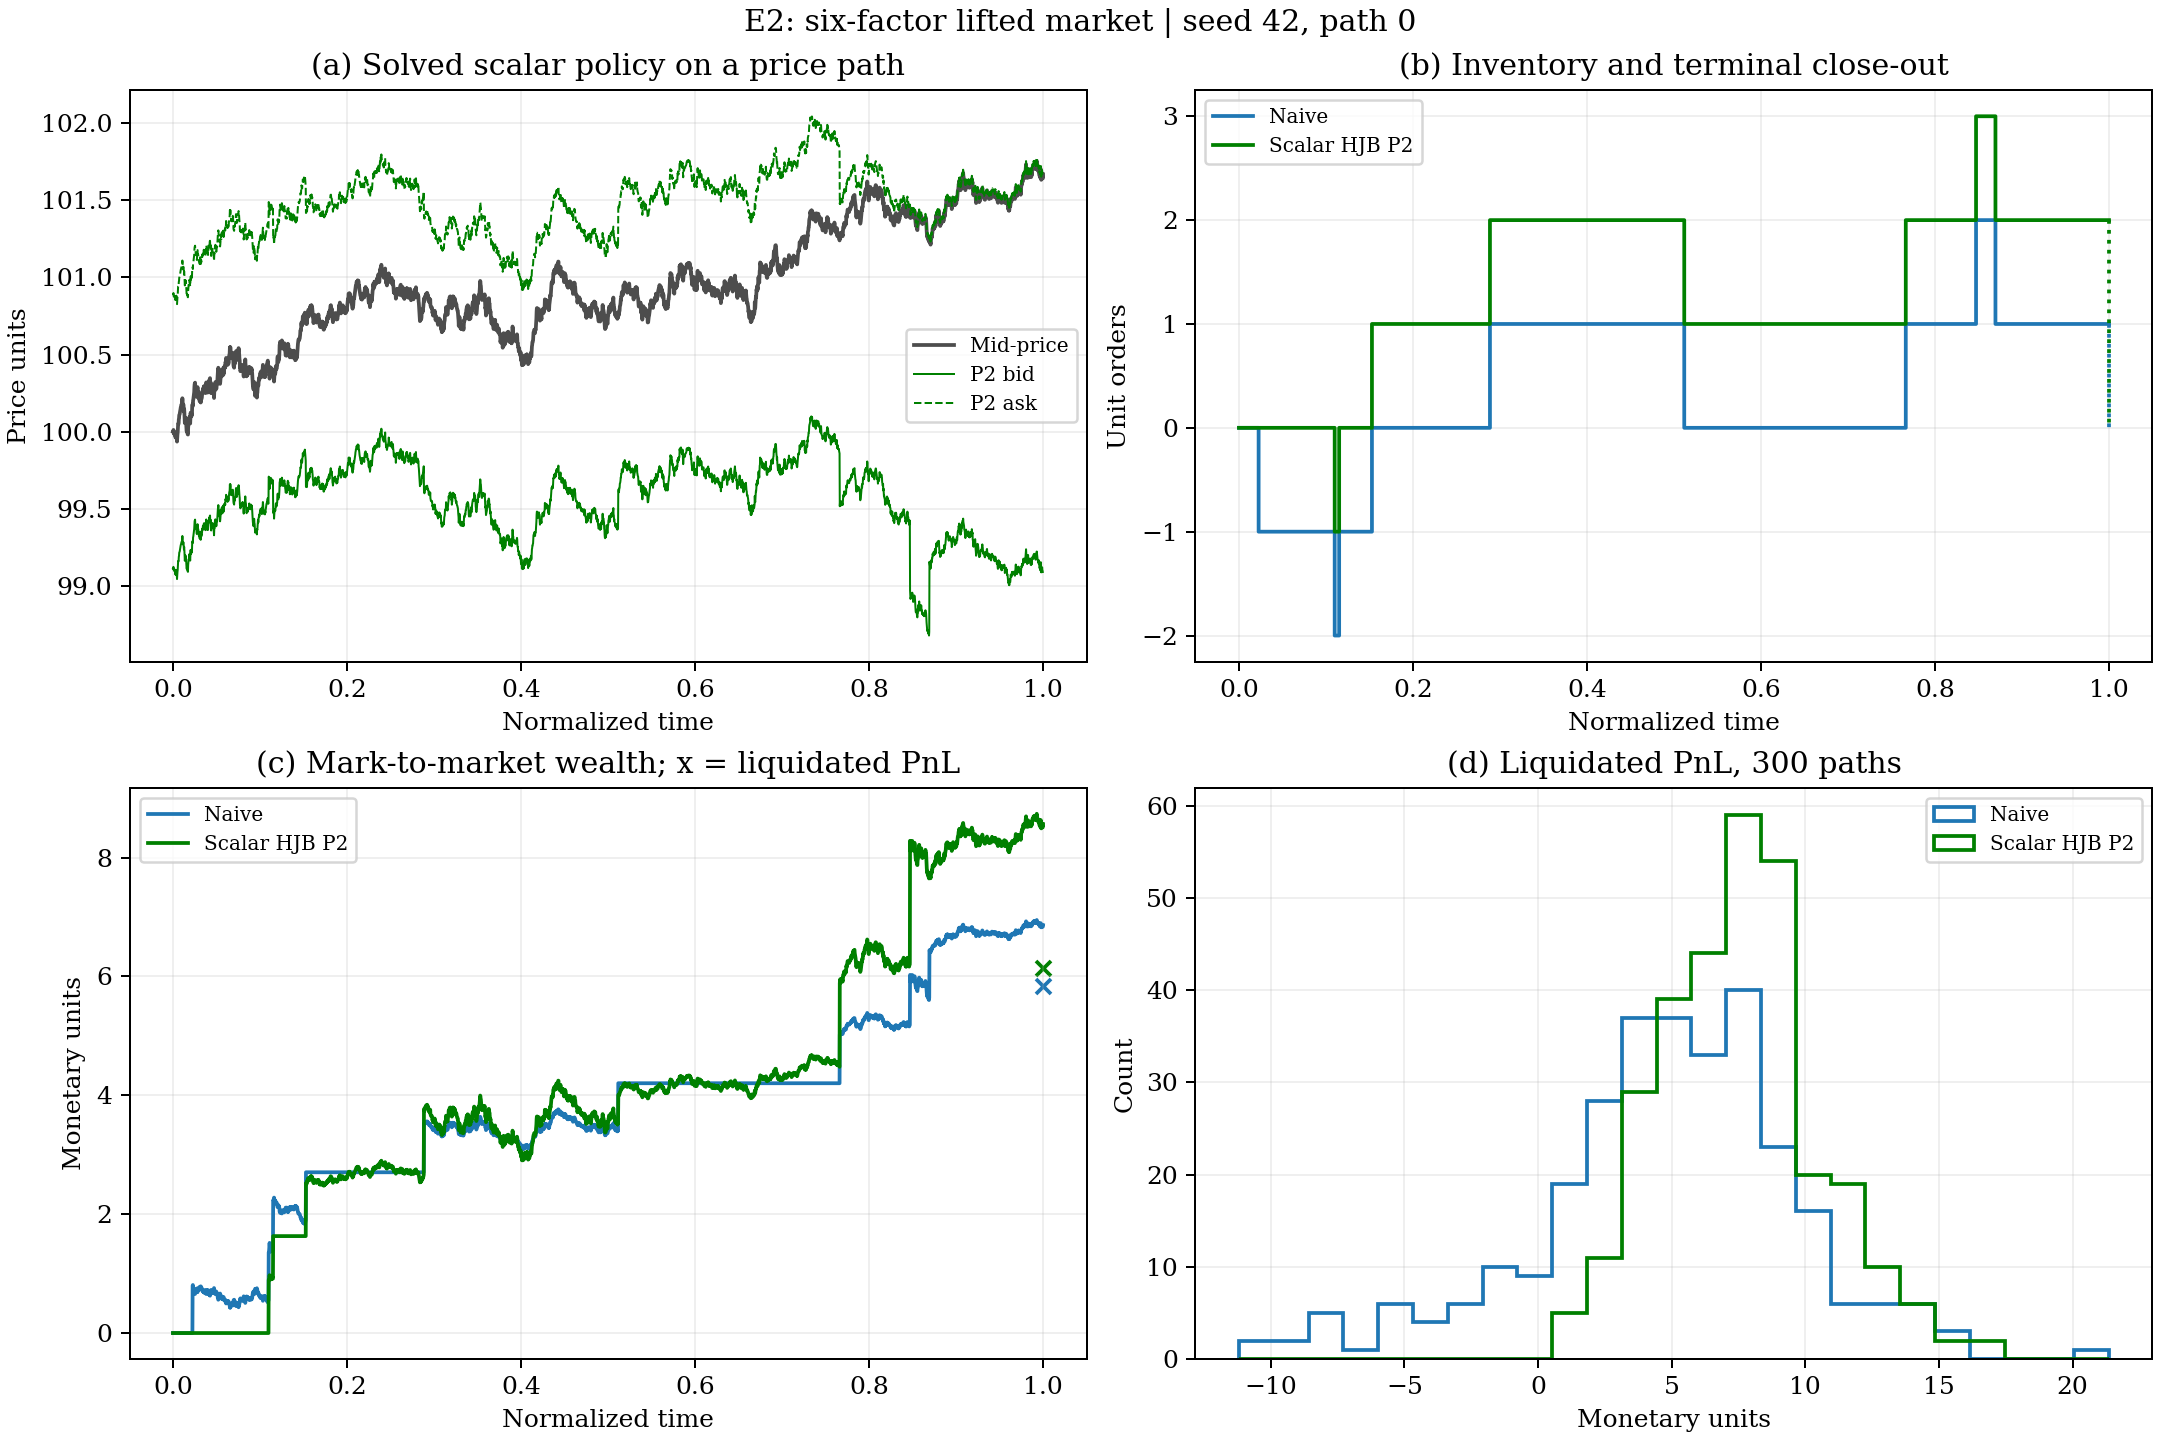
\includegraphics[width=\textwidth]{img/market_session_E2.png}
\caption{Baseline policy applied to the six-factor market E2. Top: price with P2 quotes and inventory for P2/naive. Bottom: marked wealth with liquidated terminal outcomes, and a common-bin histogram over 300 paired paths. Initial $S=100$, $X=q=0$, $T=1$, 3900 intervals, seed 42. This is P2 applied to a lifted environment, not a fitted HFT3 correction.}
\label{fig:market-e2}
\end{figure}

For E1, mean absolute inventory before liquidation is 2.433 for naive and 0.450 for P2; mean liquidated PnL is 5.445 and 7.724. For E2, these figures are 2.613 versus 0.427 and 4.792 versus 7.607. The mean paired PnL difference is 2.279 (standard error 0.215) in E1 and 2.816 (standard error 0.240) in E2. Comparisons are within each environment, not between the two sets of random paths. These synthetic baseline results do not demonstrate a correction benefit, global optimality or computational efficiency.

Checks enforce inventory limits, side disabling, exact-grid interpolation and the cash/inventory accounting identity, with maximum floating-point discrepancy $1.28\times10^{-13}$. No lookup leaves the exported state domain in these runs. The nearly singular OU innovation covariance is factored spectrally, removing only roundoff-negative eigenvalues: reconstruction error is $4.34\times10^{-19}$. The independent HJB residual, interpolation refinement and simulation-step convergence remain open. Consequently this experiment is an illustrative application, not the final validation gate for fitting P3.

\clearpage
\chapter{Multiple Assets with Multiple Volatility Factors}
\miniabstract{The preceding experiment traded one asset whose volatility had six factors. We now trade two assets, each with six factors, and let each quote depend on both inventories. A transparent covariance correction reduces average integrated risk in the first experiment, but also lowers mean PnL. It is a baseline extension, not yet the fitted residual correction proposed in this paper.}

\section{Two inventories, twelve volatility states}
Asset dimension and factor dimension have different roles. The inventory vector is $q=(q_A,q_B)$: it counts the two instruments that can be bought or sold. The volatility state is
\[
 Z=(Z_{A,1},\ldots,Z_{A,6},Z_{B,1},\ldots,Z_{B,6}).
\]
Its twelve coordinates describe persistent and rapidly decaying volatility components. They are not twelve tradable assets. Each asset has its own aggregate $Y_i=\sum_{m=1}^6w_mZ_{i,m}$ and volatility $\sigma_i(Y_i)$.

The two lifts use the same six rates, geometrically spaced between 3 and 180, with normalized weights $w_m\propto\lambda_m^{-0.7}$. Their marginal parameters match the existing scalar export, permitting reuse of its lookup tables without an additional calibration claim. The processes are
\[
 dZ_{i,m}=-\lambda_m Z_{i,m}\,dt+dB_i,
 \qquad d\langle B_A,B_B\rangle_t=\nu\,dt,\quad \nu=0.35.
\]
Within an asset, the six factors share a Brownian driver but filter its history at different rates. Across assets, the drivers are correlated rather than identical. Conditional price dynamics are
\[
 dS_i=\sigma_i(Y_i)\,dW_i,\qquad
 d\langle W_A,W_B\rangle_t=\rho\,dt,\quad \rho=0.7,
\]
with the price Brownian vector independent of the volatility Brownian vector. Thus $\nu$ controls common volatility shocks, whereas $\rho$ controls contemporaneous price shocks. Neither is inferred from the other. We retain
\[
 \sigma_i(Y_i)=1.1\exp\!\left[\frac12\left(0.75Y_i-
 \frac{0.75^2}{2}\operatorname{Var}(Y_i)\right)\right].
\]
The instantaneous covariance of price changes is
\[
 \Sigma(Y)=\begin{pmatrix}
 \sigma_A^2 & \rho\sigma_A\sigma_B\\
 \rho\sigma_A\sigma_B & \sigma_B^2
 \end{pmatrix}.
\]
Here $\rho$ is constant but $\Sigma$ is stochastic. This is not a stochastic-correlation model. Figure~\ref{fig:multi-vol} separates the twelve factor paths from the resulting two volatilities and the covariance. Assets A and B are synthetic; the experiment does not estimate the correlation of any actual pair of companies.

\begin{figure}[htbp]
\centering
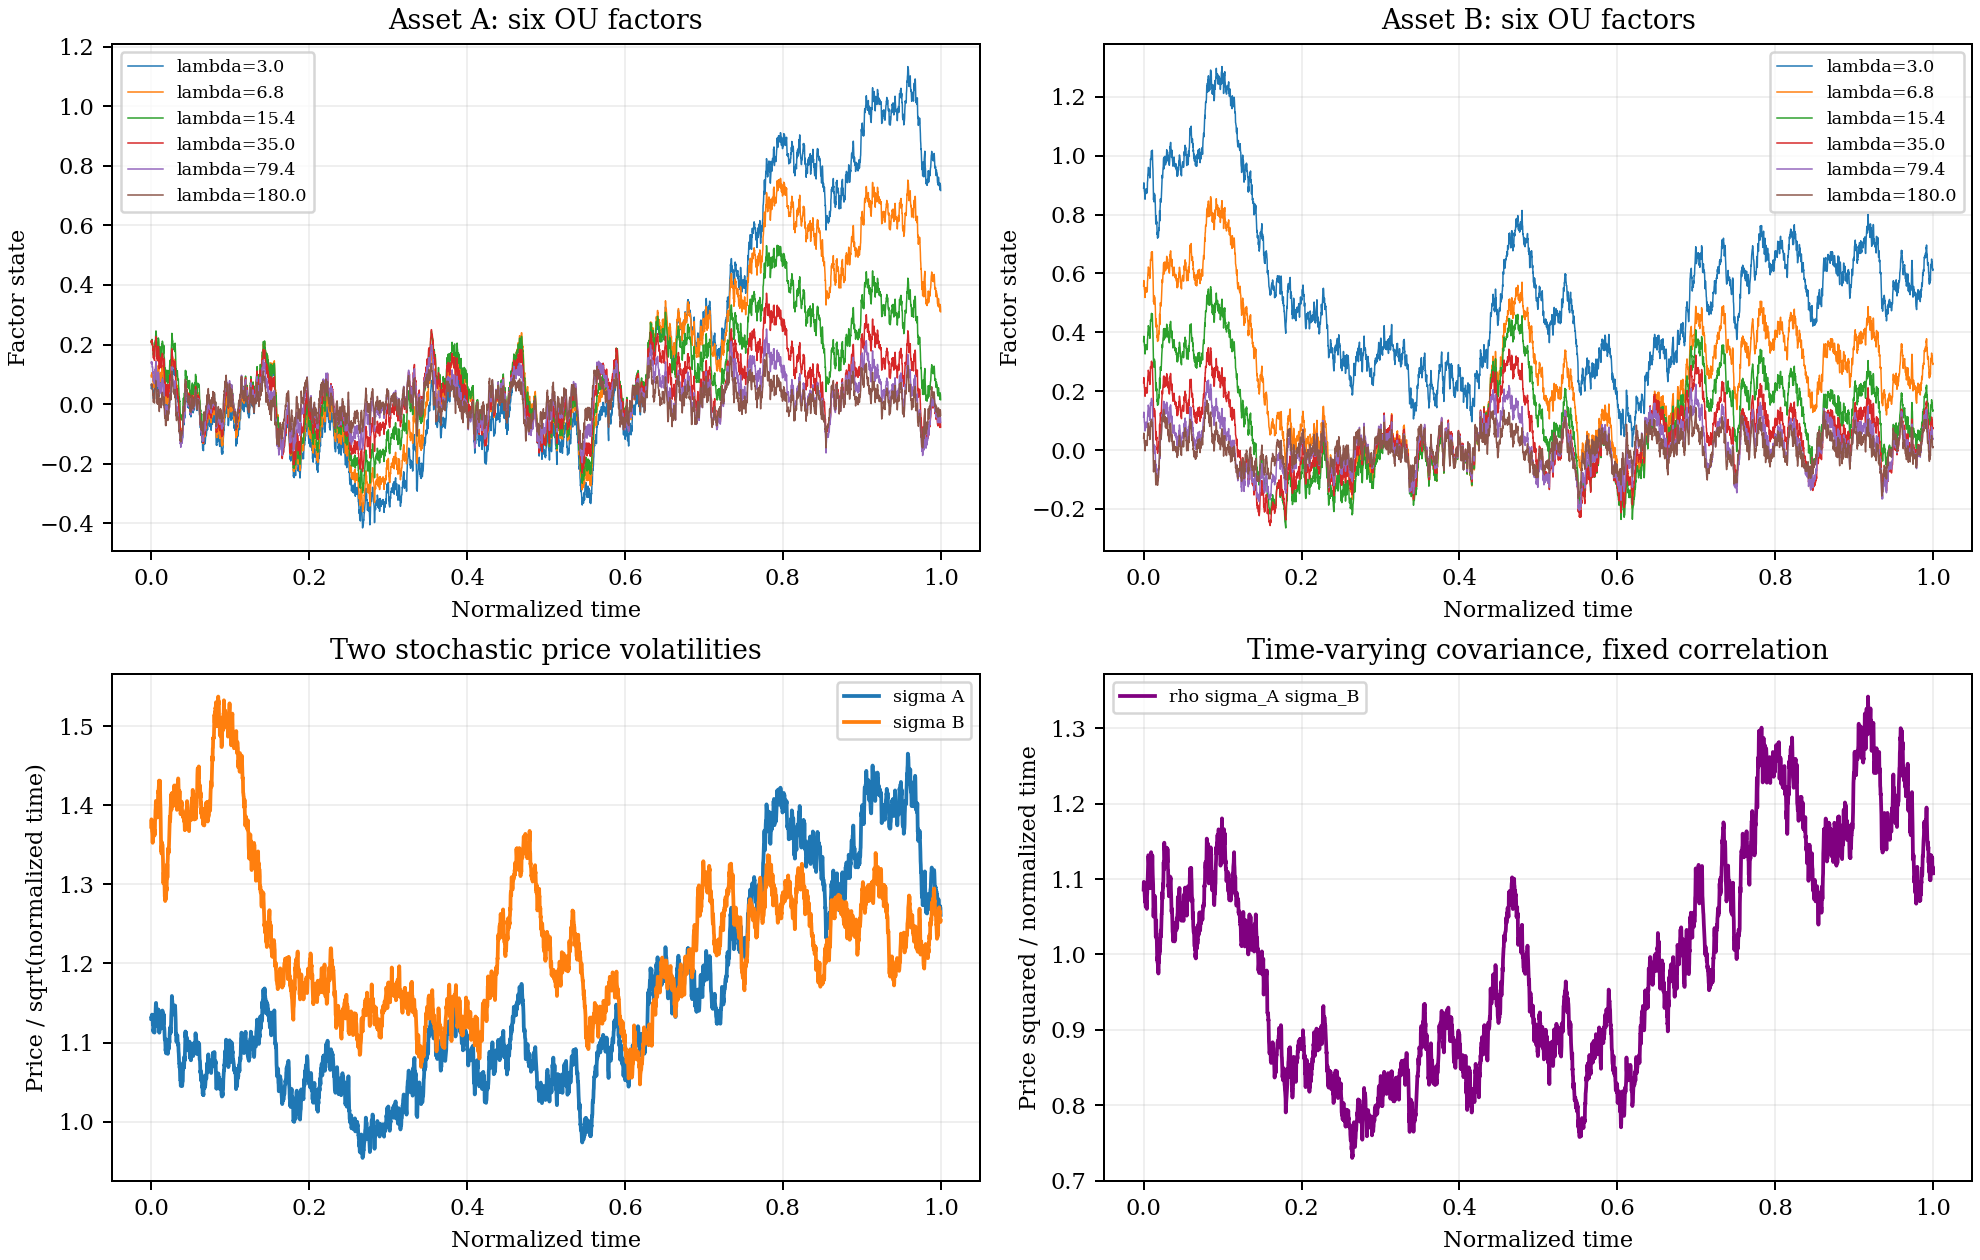
\includegraphics[width=\textwidth]{img/multiasset_volatility.png}
\caption{Two assets with six volatility factors each. Top panels show the two lifts; bottom panels show their distinct price volatilities and $\Sigma_{AB}=\rho\sigma_A\sigma_B$. Seed 73, path zero, stationary initial factor distribution, 3900 time intervals. Equal marginal parameters do not imply equal realized volatility paths.}
\label{fig:multi-vol}
\end{figure}

Exact innovations for the twelve-dimensional lift use
\[
 Q_{(i,m),(j,n)}=\nu_{ij}
 \frac{1-e^{-(\lambda_m+\lambda_n)\Delta t}}{\lambda_m+\lambda_n},
 \qquad \nu_{AA}=\nu_{BB}=1,\quad \nu_{AB}=0.35.
\]
The covariance is nearly singular for small steps. A spectral factorization removes only negative eigenvalues attributable to rounding, with a guard against a materially indefinite matrix. The maximum reconstruction discrepancy in the main run is $9.76\times10^{-19}$. This validates the factorization arithmetic, not the complete simulation discretization.

\section{How another asset's inventory changes a quote}
The variance rate of marked portfolio wealth is
\[
 \mathcal V(q,Y)=q^\top\Sigma(Y)q
 =q_A^2\sigma_A^2+q_B^2\sigma_B^2
 +2q_Aq_B\rho\sigma_A\sigma_B.
\]
With positive correlation, opposite-sign positions make the cross term negative. A short B position can therefore offset part of a long A exposure. The relevant object is this total risk, not the absolute inventory of either asset alone. For a unit sale of B, the exact change at fixed covariance is
\[
 \mathcal V(q-e_B,Y)-\mathcal V(q,Y)
 =-2(\Sigma q)_B+\Sigma_{BB}.
\]
Consequently the next sale reduces instantaneous risk only when $(\Sigma q)_B>\Sigma_{BB}/2$. The covariance benefit does not justify unlimited shorting. Finite order size, own-asset exposure, bounds and liquidation all matter. For example, at equal unit volatilities and $\rho=0.7$, moving from $(3,0)$ to $(3,-1)$ reduces the variance rate from 9 to 5.8; moving from $(3,-6)$ to $(3,-7)$ instead increases it, even before enforcing the inventory limit.

Multi-asset quoting and computational approximations are established research directions~\cite{multiapprox,multifactor}. To isolate the mechanism with our existing numerical baseline, start from the separable value
\[
 \theta_{\rm sep}(t,q,Y)
 =\theta_0(t,q_A,Y_A)+\theta_0(t,q_B,Y_B).
\]
It ignores cross-asset inventory risk in its quote calculation. The first explicit correction is
\[
 C_{\rm cov}(t,q,Y)=-\gamma(T-t)\Sigma_{AB}(Y)q_Aq_B,
 \qquad \theta_{\rm cov}=\theta_{\rm sep}+C_{\rm cov}.
\]
This approximates the omitted integrated cross-risk by freezing the current covariance over the remaining horizon. It is not an exact expectation of future covariance, and it does not solve the joint control problem. It vanishes at $T$, preserving the separable terminal liquidation cost.

Define $s_B=\gamma(T-t)\Sigma_{AB}q_A$. Buying one unit of B changes the correction by $-s_B$, while selling one changes it by $+s_B$. Since the unbounded optimal offset equals the zero-gain offset minus the neighboring-inventory gain, the implementation adds $s_B$ to the raw bid offset and subtracts $s_B$ from the raw ask offset, then applies the declared bounds. Asset A uses the symmetric expression $s_A=\gamma(T-t)\Sigma_{AB}q_B$. Applying the correction before clipping avoids losing the original gain when the baseline control is already at a bound.

If $q_A>0$ and $\rho>0$, the B ask can therefore move downward relative to the separate policy: the dealer accepts a lower selling price because the fill can offset portfolio exposure. Its B bid also moves downward, discouraging further purchases. This is a change relative to the separate quote, not a promise to sell below the mid-price, nor a guaranteed execution. Figure~\ref{fig:multi-shift} makes the sign change with correlation and inventory visible while holding all other inputs fixed.

\begin{figure}[htbp]
\centering
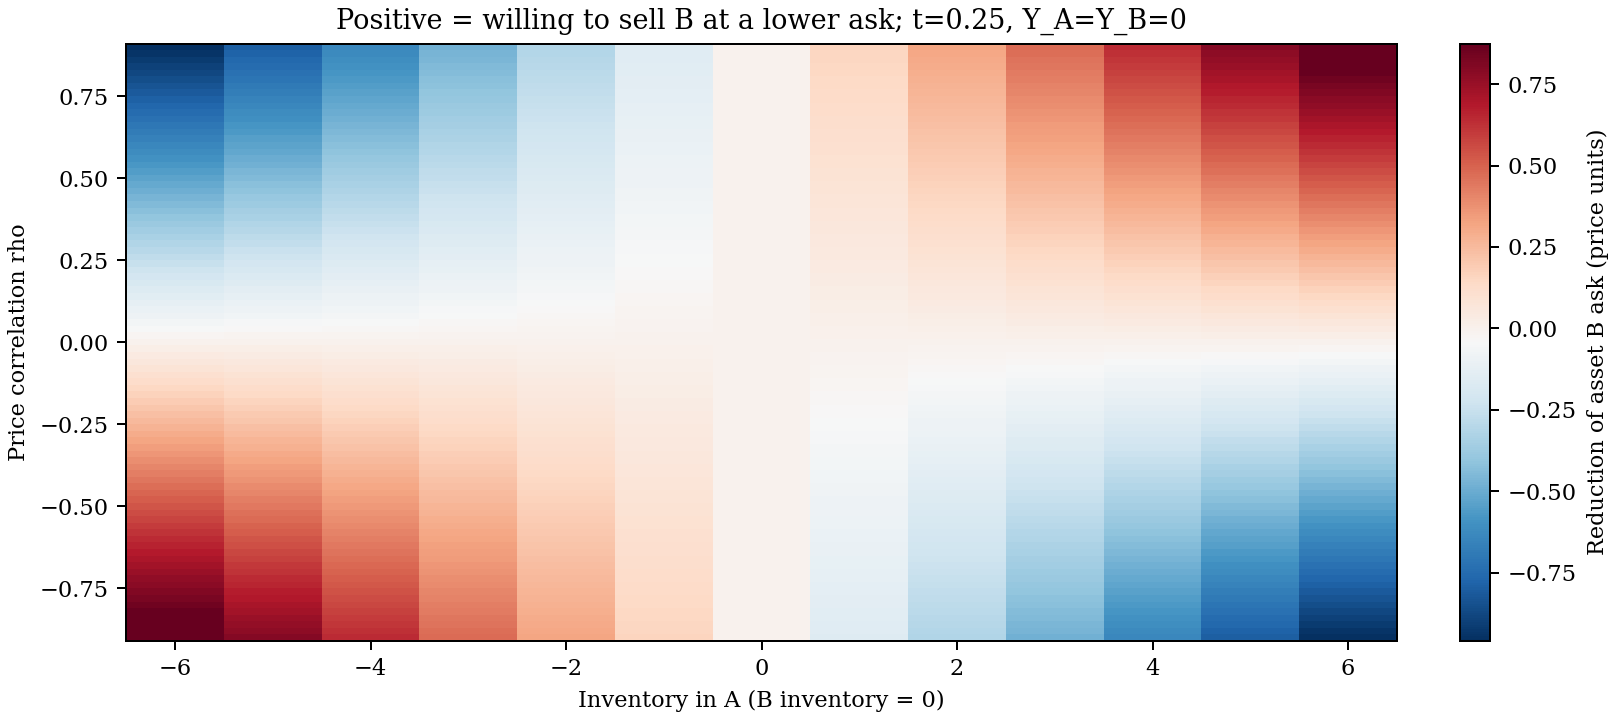
\includegraphics[width=\textwidth]{img/multiasset_quote_shift.png}
\caption{Reduction of asset B's ask relative to the separate policy, with $q_B=0$, $Y_A=Y_B=0$ and $t=0.25$. Positive values indicate a lower ask. The map varies price correlation and A inventory, using actual interpolated baseline gains and bounded controls. Zero correlation removes this explicit correction; negative correlation reverses its direction.}
\label{fig:multi-shift}
\end{figure}

\section{Joint simulations and the risk--revenue trade-off}
Both strategies begin with $q=(3,0)$, prices $(100,100)$ and cash $-300$, so initial marked wealth is zero. This deliberately exposes the cross-asset response to a long A position. For each asset the inventory limit is six units and the arrival parameters remain $A=14$, $k=1.15$. One marked Poisson candidate stream of total rate 56 chooses asset and side uniformly; acceptance probability is $e^{-k\delta}$. Inventory and both assets' quotes are updated after every accepted candidate. Common candidates and exogenous shocks pair the two policies. Price and volatility remain frozen during each interval's arrivals, followed by diffusion updates. All assets are liquidated at $T$ and the sum of the two declared liquidation costs is charged once.

Figure~\ref{fig:multi-inventory} shows path zero under seed 73, fixed independently of the outcomes. Purple B inventory initially becomes short while A is long. Later, when positions and prices have evolved differently, the same policy can carry more risk than the separate policy. The selected path is illustrative; it is not required to exhibit the average ranking at every time.

\begin{figure}[p]
\centering
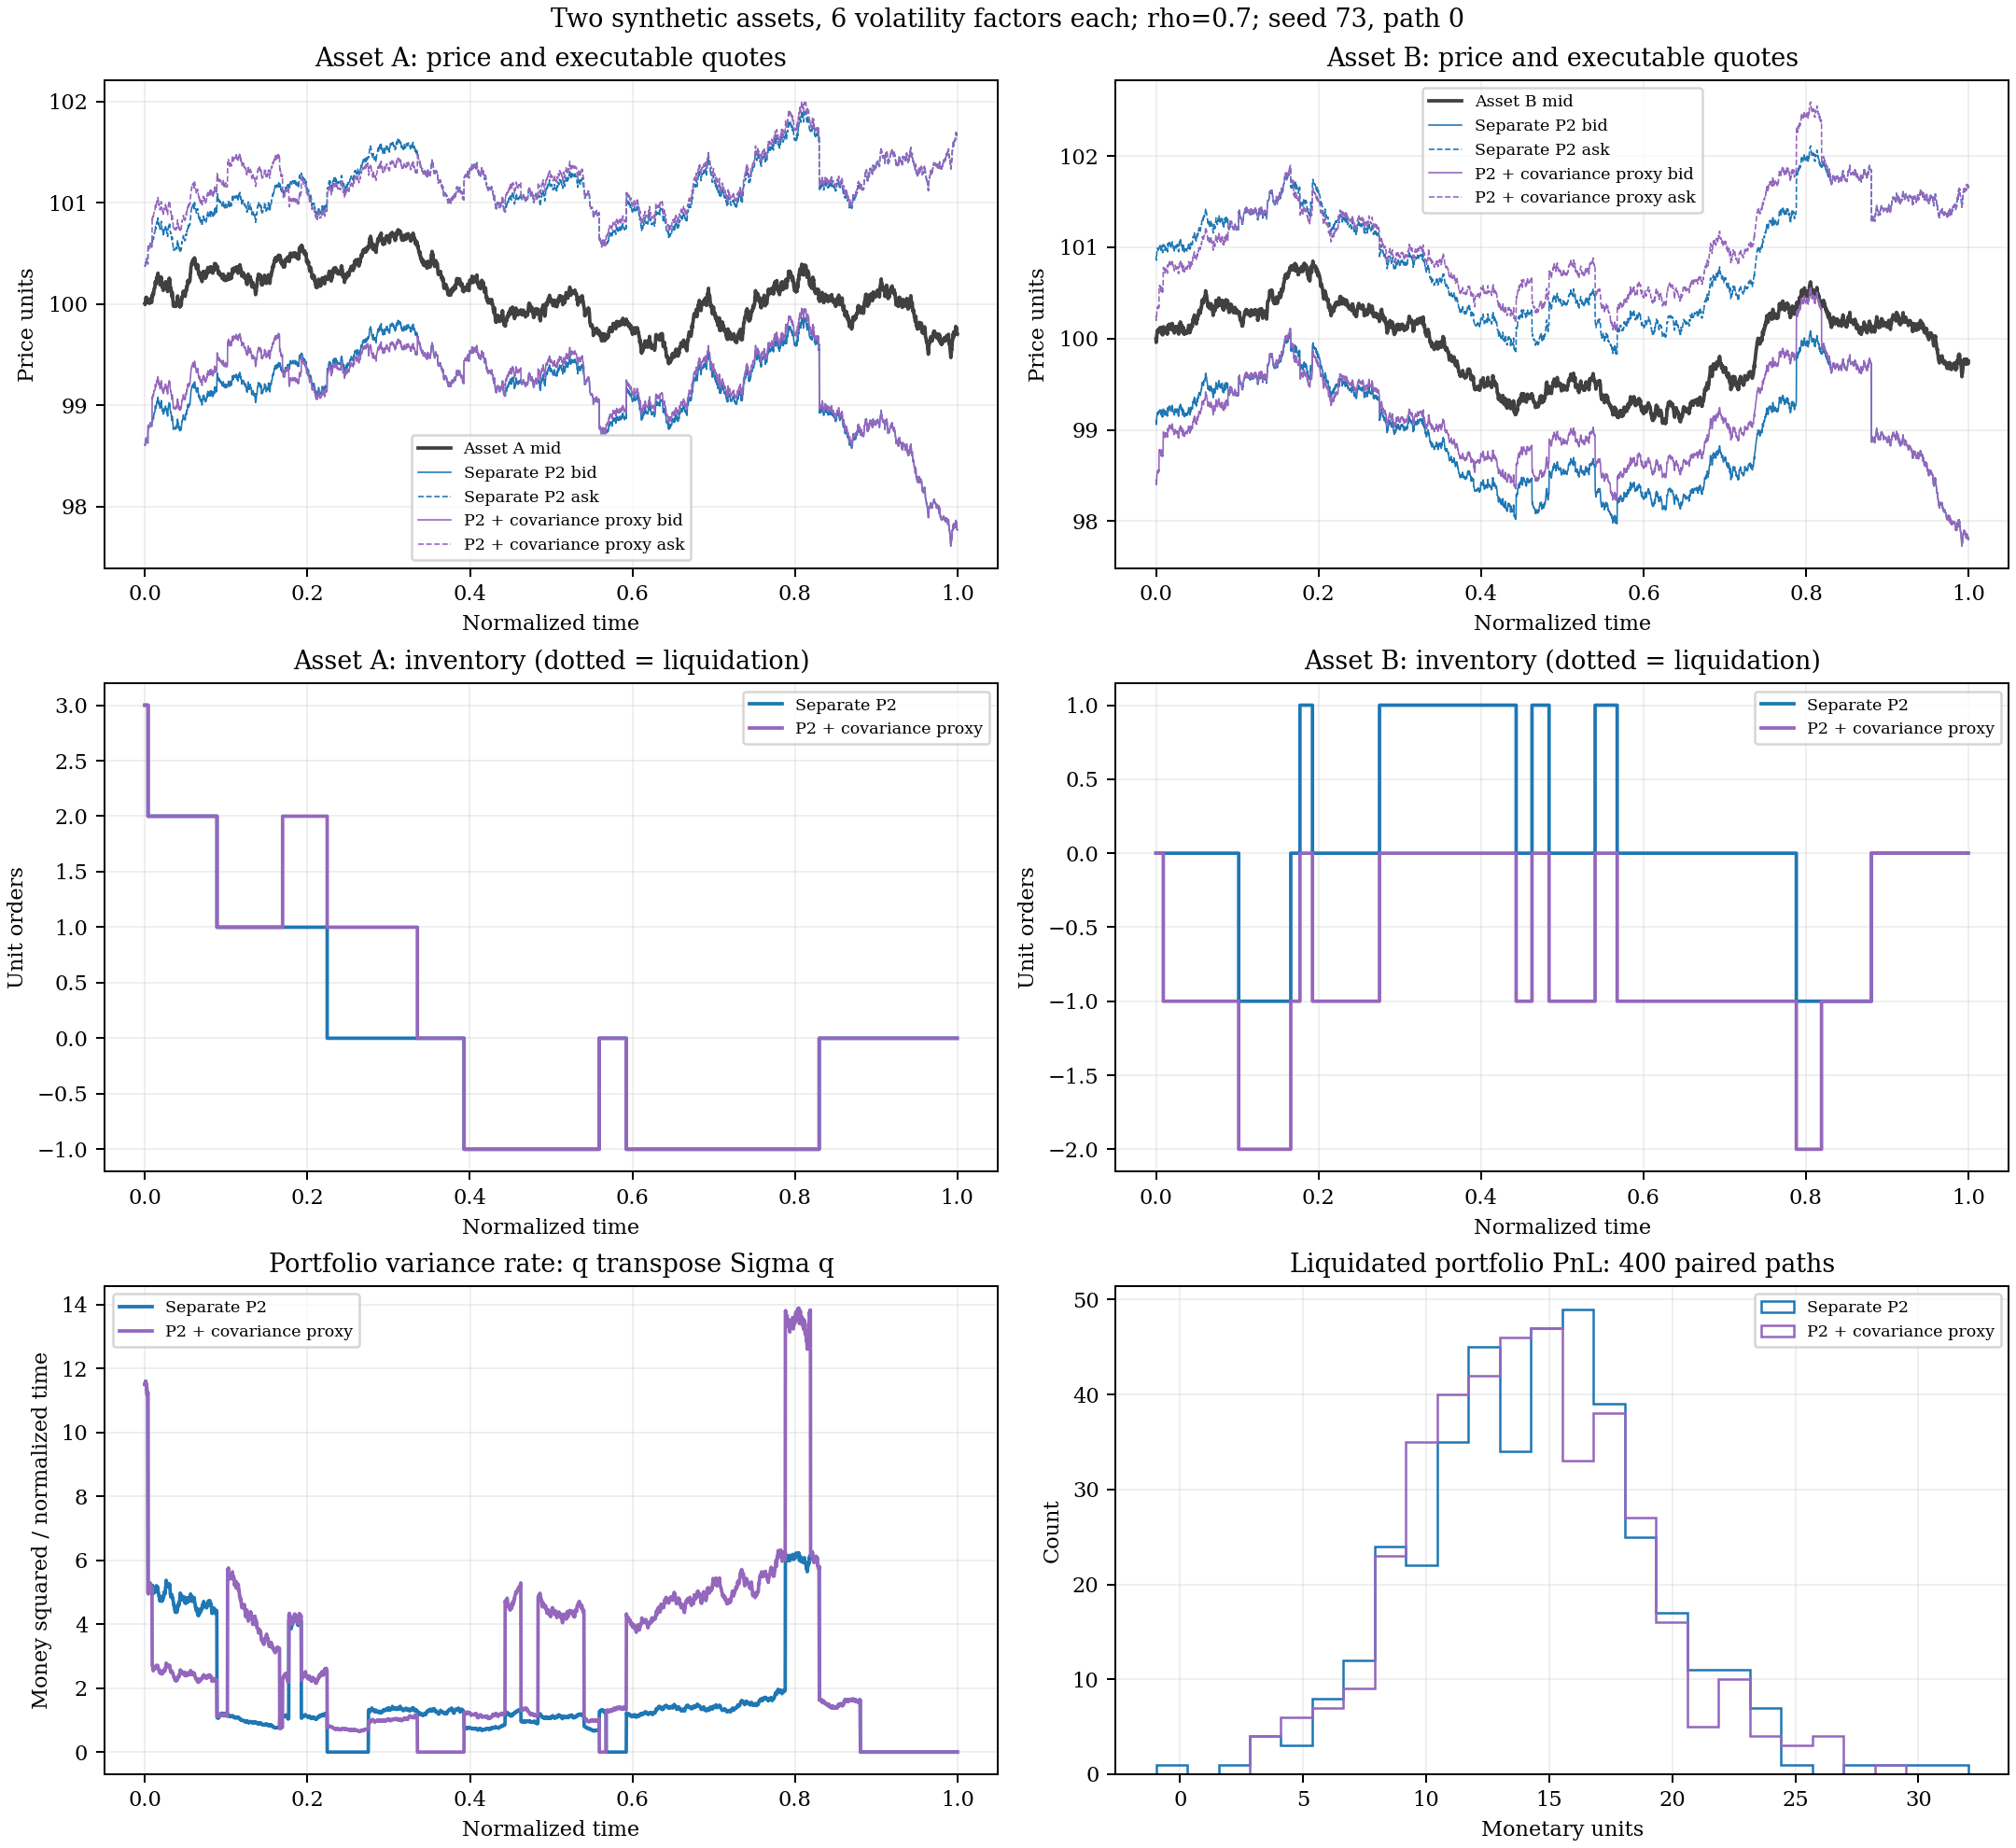
\includegraphics[width=\textwidth]{img/multiasset_inventory.png}
\caption{Two-asset application of separate P2 and P2 plus the covariance proxy. Top: both price paths and executable quotes. Middle: both inventories, with terminal liquidation dotted. Bottom: portfolio variance rate on the fixed illustrative path and liquidated PnL over 400 paired paths. Main run: 3900 intervals, price correlation 0.7, volatility-driver correlation 0.35, seed 73. The proxy is not the fitted residual-corrected policy P3.}
\label{fig:multi-inventory}
\end{figure}

For the main 400-path experiment, the results are
\begin{center}
\begin{tabular}{@{}lrr@{}}
\toprule
Metric & Separate P2 & Covariance proxy\\
\midrule
Mean $\int_0^Tq_t^\top\Sigma_tq_t\,dt$ & 5.8443 & 4.9608\\
Mean liquidated PnL & 14.4335 & 14.0905\\
Sample CARA certainty equivalent & 12.3054 & 12.2345\\
Mean $|q_A|$ before liquidation & 0.5275 & 0.5300\\
Mean $|q_B|$ before liquidation & 0.4825 & 0.5200\\
\bottomrule
\end{tabular}
\end{center}
The integrated-risk difference (proxy minus separate) is $-0.8835$, with paired standard error 0.1085: approximately 15.1\% lower mean integrated variance. This metric measures accumulated instantaneous inventory risk, not the sample variance of terminal PnL. The mean PnL difference is $-0.3430$, with paired standard error 0.0908. The sample certainty equivalent $-\log(\operatorname{mean}e^{-\gamma\mathrm{PnL}})/\gamma$ also decreases slightly; no confidence interval for that nonlinear statistic has been computed. The experiment therefore does not establish an improvement in the CARA objective. It shows a risk--revenue trade-off and motivates a better correction rather than validating this proxy as optimal.

A 1950-interval diagnostic with 400 paths has the same qualitative average trade-off: integrated variance 5.9781 versus 5.2543, PnL 13.9323 versus 13.6632. These two resolutions do not certify convergence. Reusing a seed at a different step count does not couple identical Brownian paths across resolutions; pairing is within each run. A separate zero-price-correlation regression produces identical inventories, cash and outcomes for both policies, even though the volatility drivers retain correlation 0.35. Thus this correction isolates price-covariance inventory coupling, not every source of dependence.

\section{From a covariance proxy to a full residual correction}
The full lifted operator now has two inventory coordinates and twelve volatility coordinates. With $a$ the instantaneous covariance of the factor drivers and $\mathcal L_Z$ their OU generator, price/factor independence gives
\begin{align*}
\mathcal H[\theta]={}&\theta_t+\mathcal L_Z\theta
-\frac{\gamma}{2}(\nabla_Z\theta)^\top a\nabla_Z\theta
-\frac{\gamma}{2}q^\top\Sigma(Z)q\\
&+\sum_{i=1}^{2}\bigl[H_i(\theta(q+e_i)-\theta(q))
+H_i(\theta(q-e_i)-\theta(q))\bigr],
\end{align*}
omitting forbidden transitions. The C++ implementation supports fixed asset and total-factor dimensions and common arrival/control parameters; its caller supplies valid covariance matrices. Tests cover cross-asset risk, mixed factor Hessians, the gradient-square term and inventory bounds. In the restricted constant-covariance, no-arrival setting, the time derivative of $C_{\rm cov}$ exactly cancels the omitted cross-risk term relative to the diagonal baseline. That algebraic check does not establish cancellation in the stochastic-volatility model.

Indeed, $C_{\rm cov}$ also has factor derivatives when $\Sigma$ is stochastic, and changes all arrival Hamiltonians through the neighboring-inventory gains. Correlated volatility drivers introduce further mixed terms. The complete residual must be recomputed with these contributions before a localized fitted correction can be accepted. No residual reduction is asserted for the proxy in the experiment above.

For $N$ assets and $K$ total factors, a tensor inventory grid already contains $(2Q+1)^N$ states before discretizing volatility. Reusing separate scalar policies avoids that joint solve, but loses coupling. The explicit pair correction requires a covariance--inventory product, costing $O(N^2)$ for a dense covariance, in addition to scalar lookups; factor simulation costs are separate. This explains the proposed computational advantage and its approximation cost. No measured speedup is reported. The next research step is to use a validated multi-asset baseline and full residual to fit and test localized corrections, retaining risk, utility and computational cost as distinct acceptance criteria.
\clearpage

\chapter{Results and Limitations}
\miniabstract{The first increment establishes a reproducible defect calculation and identifies a baseline issue. The research claims remain limited to that scope.}

The operator decomposition makes two sources of discrepancy visible: the aggregate drift is not generally a function of the scalar state alone, and stationary-variance matching does not match instantaneous diffusion. The C++ evaluator implements this declared common-noise model and agrees with an independent calculation on the exported samples.

The baseline diagnostic also shows why a residual-first workflow needs numerical discipline. If a scalar solution is heavily clipped and has a large residual in its own declared operator, a subsequent correction may be compensating for discretization artifacts. The positive transformed scheme now provides a bounded-control baseline without value clipping, with initial refinement evidence. Domain sensitivity and a residual study remain necessary before treating it as a validated reference for a correction dictionary.

Several questions remain open. No correction coefficients have been fitted. No nontrivial preservation statistic has been tested under a corrected policy. No two- or three-factor reference solution, corrected-policy Monte Carlo comparison or latency frontier has been produced. Illustrative baseline-versus-naive simulations are now available in E1 and E2; their discretization validation remains open. The exact Navier--Stokes source remains unverified. These are explicit continuation tasks rather than negative results about the proposed architecture.

\chapter*{Conclusion}
\addcontentsline{toc}{chapter}{Conclusion}
\markboth{Conclusion}{Conclusion}
HFT3 now has a defined full-HJB defect, derivative-aware correction interfaces, a reproducible audit and a positive scalar baseline with bounded controls. The first result is methodological: numerical error in the inherited reduced calculation must be separated from state-compression error before correction quality is assessed. Time-dependent export and initial domain/grid figures are now available. Subsequent work will complete residual and interpolation validation, then evaluate constrained localized corrections against policy accuracy, inventory risk and software cost. The proposed Navier--Stokes connection remains an architectural research direction pending verification of the exact source; it does not supply a theorem for the financial model.

\begin{references}
\bibitem{multiapprox} P. Bergault, D. Evangelista, O. Gu\'eant and D. Vieira, \textit{Closed-form approximations in multi-asset market making}, arXiv:1810.04383, version 5, 2022. \url{https://arxiv.org/abs/1810.04383}.
\bibitem{multifactor} P. Bergault and O. Gu\'eant, \textit{Size matters for OTC market makers: general results and dimensionality reduction techniques}, arXiv:1907.01225, version 5, 2022. \url{https://arxiv.org/abs/1907.01225}.
\bibitem{as} M. Avellaneda and S. Stoikov, \textit{High-frequency trading in a limit order book}, Quantitative Finance 8(3), 217--224, 2008. \url{https://math.nyu.edu/inmemoriam/avellaneda/HighFrequencyTrading.pdf}.
\bibitem{hft1} S. G. Messina and N. Soriano, \textit{High-Frequency Market Making under Avellaneda--Stoikov}, Starting Finance Club PoliTo, Research, published article supplied to this project.
\bibitem{hft2} S. G. Messina and N. Soriano, \textit{Rough Volatility and End-of-Day Inventory Control}, Starting Finance Club PoliTo, Research, unpublished working manuscript supplied to this project.
\bibitem{code} S. G. Messina, \textit{Residual-Corrected Rough-Volatility HJBs: supporting code}, Starting Finance Club PoliTo, Research, GitHub repository, \texttt{INSERIRE LINK GITHUB}. Working version, 9 September 2026.
\end{references}


